\documentclass[english,12pt,a4paper]{report}
\usepackage[utf8]{inputenc}
\usepackage[T1]{fontenc}
\usepackage{babel}
\usepackage{amssymb}
\usepackage{graphicx}
\usepackage{mathtools}
\usepackage{nameref}
\usepackage[hidelinks]{hyperref}
\usepackage{enumitem}
\usepackage{tabularx}


\makeatletter
\def\@makechapterhead#1{
	\vspace*{0\p@}
	{\parindent \z@ \raggedright \normalfont
		\interlinepenalty\@M
		\Huge \bfseries #1\par\nobreak
		\vskip 40\p@
}}


\begin{document}
	\begin{titlepage}
		\centering
		\Huge
		\textbf{PROJECT REPORT}\\
		\vspace{1cm}
		\textbf{METRICSTICS}\\
		\textbf{(DELIVERABLE - 1)}\\
		\vspace{1.5cm}
		\Large
		\textbf{Prepared By}\\
		\vspace{0.5cm}
		Sharanyu Pillai(40227794)\\
		Wei Qi(40198872)\\
		Anitha Ramakrishnan(40231724)\\
		Arshiya Sahni(40202614)\\
		Vinay Sahrawat(40220936)\\
		\vspace{1.5cm}
		\large
		\textbf{Under the Guidance of}\\
		Prof. Pankaj Kamthan \\
		\vspace{1.5cm}
		\textbf{Submitted at}\\
		CONCORDIA UNIVERSITY\\
		\centering
		
\includegraphics[width=8cm]{concordia.jpg}
		\vfill
		Github:\\
		\url{https://github.com/WeiQi5588/SOEN-6611} \\
		By Team M
		\thispagestyle{empty} 
	\end{titlepage}
	
	\newpage 
	\setcounter{page}{0}
	\pagenumbering{gobble}
	\tableofcontents
	\clearpage
	
	\pagenumbering{arabic}
	

	
	\chapter{Introduction}

	 There has been a growing recognition of the pivotal role that descriptive statistics play in data analysis. Descriptive statistics provide a quantitative framework for characterizing the features of a dataset. By employing measures of central tendency, frequency distributions, and variability, descriptive statistics offer valuable insights into the underlying structure and patterns within the data, laying the groundwork for further analysis and interpretation. In this context, we consider a random variable denoted as x, which draws values from a finite dataset {x1, x2, x3, ..., xn}, where each value carries an equal probability. Within this framework, we introduce the concepts of minimum (m) and maximum (M), representing the smallest and largest values in the dataset, respectively. Additionally, we identify the mode (o) as the value with the highest frequency. For measures of central location, we introduce the median (d), which represents the middle value when the dataset size is odd, and the arithmetic mean when it is even.
	\section{System Information}
	A key system is being developed as part of the development of the Logistics and Supply Chain 	Analytics Solution, known as "METRICSTICS," to conduct a thorough study of logistics and supply chain performance. This system will examine statistical analyses of logistical data with the goal of giving the logistics management team the tools they need to efficiently track trends in logistics operations over time. It will enable thorough examinations of historical records in the logistics and supply chain area, enabling well-informed decision-making based on the priceless insights gained. Professionals in logistics, such as Warehouse Manager, Logistics Managers, Inventory managers and Procurement Managers, make up the majority of "METRICSTICS"'s stakeholders and will gain the most from the insights and features this analytics solution provides.
	
	\section{Assumptions}
	The project has the following assumptions:
	\begin{enumerate}
	\item \textbf{Random Variables and Data Set} 
	\begin{itemize}
		\item The system operates on random variables that can take values from a finite data set $x_1, x_2, x_3, \ldots, x_n$ with each value having the same probability.
	\end{itemize}

	\item \textbf{Probability Distribution:} 
	\begin{itemize}
	\item The probability distribution of the random variable is assumed to be uniform, as each value in the data set has the same probability.
	\end{itemize}
	
	\item \textbf{Uniqueness of Minimum and Maximum:} 
	\begin{itemize}
		\item The probability distribution of the random variable is assumed to be uniform, as each value in the data set has the same probability.
	\end{itemize}

	\item \textbf{Uniqueness of Mode:} 
	\begin{itemize}
	\item The mode $o$ may not be unique. There can be multiple modes if multiple values occur with the highest frequency.
	\end{itemize}
	
	\item \textbf{Calculation of Median for Even $n$:} 
	\begin{itemize}
		\item When the number of observations ($n$) is even, the median $d$ is calculated as the arithmetic mean of the two middle values.
	\end{itemize}

	\item \textbf{Calculation of Standard Deviation:} 
	\begin{itemize}
	\item The standard deviation ($\sigma$) is calculated based on the squared differences between each observation and the arithmetic mean.
	\end{itemize}

	\item \textbf{Accuracy of Data:} 
	\begin{itemize}
	\item It is assumed that the data provided to the system is accurate and free from errors.
	\end{itemize}

	\item \textbf{Input Data Source:} 
	\begin{itemize}
		\item The system can accept data from different sources, including real-world data from authoritative sources or artificially generated data from a random data generator.
	\end{itemize}
	\end{enumerate}
	
	\section{Constraints}
	The project has some potential constraints:
	\begin{enumerate}
		
	\item \textbf{Computational Resources:} 
	\begin{itemize}
		\item The system's performance may be limited by the available computational resources, such as processing power, memory, and storage.
	\end{itemize}

	\item \textbf{Input Data Quality:} 
	\begin{itemize}
		\item The accuracy and reliability of the descriptive statistics may be affected by the quality and integrity of the input data. Inaccurate or incomplete data may lead to unreliable results.
	\end{itemize}

	\item \textbf{Data Size:} 
	\begin{itemize}
		\item The system may face limitations in processing very large datasets, potentially leading to longer processing times or resource constraints.
	\end{itemize}

	\item \textbf{Statistical Assumptions:} 
	\begin{itemize}
		\item The accuracy of the descriptive statistics relies on the validity of certain statistical assumptions, such as the assumption of a uniform probability distribution for the data.
	\end{itemize}
	
	\item \textbf{Output Interpretation:} 
	\begin{itemize}
		\item Users must be able to interpret the descriptive statistics correctly to derive meaningful insights from the results. Inadequate understanding may lead to misinterpretation.
	\end{itemize}

	\end{enumerate}
	
	\chapter{Problem 1: Goal-Question-Metric}
		\section{Goal}
\begin{tabular}{|p{14cm}|}
	\hline
	\\
	\textbf{Purpose} \\
	To conduct a comprehensive analysis of historical logistics and supply chain data to gain a deep understanding of the trends and patterns that have evolved over time. \\
	\\
	\textbf{Perspective} \\
	Assess the historical logistics and supply chain data from the viewpoint of logistics and supply chain management. \\
	\\
	\textbf{Environment} \\
	Within the context of developing the Logistics and Supply Chain Analytics Solution (METRICSTICS). \\
	\\
	\hline
\end{tabular}

\section{SMART Principles}
The goal is considered SMART (Specific, Measurable, Attainable, Realistic, and Timely) for the following reasons:
\begin{itemize}
	\item \textbf{Specific:} The METRICSTICS program is particularly specific in that it specifically defines the goal of examining historical logistics and supply chain data to get a thorough understanding of trends and patterns within the area. This focus enables us to give specific and meaningful information to logistics and supply chain managers, allowing informed decision-making.
	
	\item \textbf{Measurable:} The project's success is measurable through the formulation of key performance indicators and questions. These indicators could include measures of annual logistics cost reduction, inventory turnover rates, on-time delivery performance, and supply chain cycle time reduction. We can assess the influence of METRICSTICS by quantifying these aspects.
	
	\item \textbf{Attainable:} The aim is Attainable, as the application of METRICSTICS allows for the examination of past logistics and supply chain data. METRICSTICS equips logistics professionals with the necessary tools and infrastructure to collect, process, and analyze pertinent data, ultimately providing them with important insights.
	
	\item \textbf{Realistic:} The goal of METRICSTICS is realistic in relation to the jobs and responsibilities of logistics and supply chain management. It allows them to obtain a thorough understanding of previous performance, optimize logistics and supply chain strategies, and set realistic goals for future improvements. As a result, METRICSTICS skills are perfectly aligned with the requirements of logistics experts.
	
	\item \textbf{Timely:} The project is Timely since it focuses on the study of historical logistics and supply chain data spanning certain time periods, ensuring a well-defined timeframe for completing analyses. This approach ensures that we stay on track to achieve our goal within the designated timeframe and budget.
\end{itemize}
In brief, METRICSTICS follows the SMART principles of being Specific, Measurable, Attainable, Realistic, and Timely. These criteria lead our efforts to provide an analytics solution that is well-defined, quantifiable, realistic, applicable, and time-bound for logistics and supply chain professionals.

\section{Question And Metric}
\begin{itemize}[align=left, left=0em,labelsep=0em]
	\item[\textbullet\ ] \textbf{Question 1:} What is the average supplier delivery cost for stock on a monthly and quarterly basis?
	\begin{itemize}[align=left, left=0em,labelsep=0em]
		\item[] \textbf{Metric:}
		\begin{enumerate}[label={}, left=0em, labelwidth=1em, labelsep=0em, align=left]
			\item M1. Average monthly supplier delivery cost
			\item M2. Average quarterly supplier delivery cost
		\end{enumerate}
		\item[] \textbf{Mechanism:}
		\begin{enumerate}[label={}, left=0em, labelwidth=1em, labelsep=0em, align=left]
			\item[i.] Owner = Logistics Managers
			\item[ii.] Frequency Collected = Following procurement data entry
			\item[iii.] Frequency Reported = Monthly and Quarterly
		\end{enumerate}
	\end{itemize}
	
	\item[\textbullet\ ] \textbf{Question 2:} What is the percentage change in shipping costs for each shipping method, both monthly and quarterly? 
	\begin{itemize}[align=left, left=0em,labelsep=0em]
		\item[] \textbf{Metric:}
		\begin{enumerate}[label={}, left=0em, labelwidth=1em, labelsep=0em, align=left]
			\item M3. Maximum monthly shipping cost increase percentage
			\item M4. Minimum monthly shipping cost decrease percentage
			\item M5. Maximum quarterly shipping cost increase percentage
			\item M6. Minimum quarterly shipping cost decrease percentage
		\end{enumerate}
		\item[] \textbf{Mechanism:}
		\begin{enumerate}[label={}, left=0em, labelwidth=1em, labelsep=0em, align=left]
			\item[i.] Owner = Logistics Managers
			\item[ii.] Frequency Collected = Following shipping cost data update
			\item[iii.] Frequency Reported = Monthly and Quarterly
		\end{enumerate}
	\end{itemize}
	
	\item[\textbullet\ ] \textbf{Question 3:} How do we identify fluctuations in warehouse storage space utilization on a monthly and quarterly basis? 
	\begin{itemize}[align=left, left=0em,labelsep=0em]
		\item[] \textbf{Metric:}
		\begin{enumerate}[label={}, left=0em, labelwidth=1em, labelsep=0em, align=left]
			\item M7. Calculate the Monthly Average Storage Utilization Rate
			\item M8. Calculate the Quarterly Average Storage Utilization Rate
		\end{enumerate}
		\item[] \textbf{Mechanism:}
		\begin{enumerate}[label={}, left=0em, labelwidth=1em, labelsep=0em, align=left]
			\item[i.] Owner = Warehouse Managers
			\item[ii.] Frequency Collected = Following warehouse storage data analysis
			\item[iii.] Frequency Reported = Monthly and Quarterly
		\end{enumerate}
	\end{itemize}
	
	\item[\textbullet\ ] \textbf{Question 4:} Which month and quarter experienced the most significant inventory turnover rate change over the year? 
	\begin{itemize}[align=left, left=0em,labelsep=0em]
		\item[] \textbf{Metric:}
		\begin{enumerate}[label={}, left=0em, labelwidth=1em, labelsep=0em, align=left]
			\item M9. Standard deviation of monthly inventory turnover rates
		\end{enumerate}
		\item[] \textbf{Mechanism:}
		\begin{enumerate}[label={}, left=0em, labelwidth=1em, labelsep=0em, align=left]
			\item[i.] Owner = Inventory Managers
			\item[ii.] Frequency Collected = Following inventory turnover rate analysis
			\item[iii.] Frequency Reported = Monthly and Quarterly
		\end{enumerate}
	\end{itemize}
	
	\item[\textbullet\ ] \textbf{Question 5:} Which month and quarter experienced the most significant supplier delivery time changes over the year? 
	\begin{itemize}[align=left, left=0em,labelsep=0em]
		\item[] \textbf{Metric:}
		\begin{enumerate}[label={}, left=0em, labelwidth=1em, labelsep=0em, align=left]
			\item M10. Standard deviation of monthly supplier delivery times
		\end{enumerate}
		\item[] \textbf{Mechanism:}
		\begin{enumerate}[label={}, left=0em, labelwidth=1em, labelsep=0em, align=left]
			\item[i.] Owner = Logistics Managers
			\item[ii.] Frequency Collected = Following supplier delivery time analysis
			\item[iii.] Frequency Reported = Monthly and Quarterly
		\end{enumerate}
	\end{itemize}
	
	\item[\textbullet\ ] \textbf{Question 6:} How can we identify the top 10 suppliers with the most consistent on-time deliveries on a monthly and quarterly basis? 
	\begin{itemize}[align=left, left=0em,labelsep=0em]
		\item[] \textbf{Metric:}
		\begin{enumerate}[label={}, left=0em, labelwidth=1em, labelsep=0em, align=left]
			\item M11. Count the number of times each supplier has on-time deliveries in a month and quarter
			\item M12. Sort suppliers by their on-time delivery frequency
		\end{enumerate}
		\item[] \textbf{Mechanism:}
		\begin{enumerate}[label={}, left=0em, labelwidth=1em, labelsep=0em, align=left]
			\item[i.] Owner = Logistics Managers
			\item[ii.] Frequency Collected = Following supplier performance data collection
			\item[iii.] Frequency Reported = Monthly and Quarterly
		\end{enumerate}
	\end{itemize}
	
	\item[\textbullet\ ] \textbf{Question 7:} What is the most commonly used transportation route for shipments on a monthly basis? 
	\begin{itemize}[align=left, left=0em,labelsep=0em]
		\item[] \textbf{Metric:}
		\begin{enumerate}[label={}, left=0em, labelwidth=1em, labelsep=0em, align=left]
			\item M13. Count the number of shipments on each route in a month and find the route with the highest count.
		\end{enumerate}
		\item[] \textbf{Mechanism:}
		\begin{enumerate}[label={}, left=0em, labelwidth=1em, labelsep=0em, align=left]
			\item[i.] Owner = Logistics Managers
			\item[ii.] Frequency Collected = Following shipment data analysis
			\item[iii.] Frequency Reported = Monthly
		\end{enumerate}
	\end{itemize}
	
	\item[\textbullet\ ] \textbf{Question 8:} In which region do we experience the highest number of shipping delays on a yearly basis? 
	\begin{itemize}[align=left, left=0em,labelsep=0em]
		\item[] \textbf{Metric:}
		\begin{enumerate}[label={}, left=0em, labelwidth=1em, labelsep=0em, align=left]
			\item M14. Count the number of shipping delays by region for the entire year and find the region with the highest count.
		\end{enumerate}
		\item[] \textbf{Mechanism:}
		\begin{enumerate}[label={}, left=0em, labelwidth=1em, labelsep=0em, align=left]
			\item[i.] Owner = Logistics Managers
			\item[ii.] Frequency Collected = Following yearly shipping delay analysis
			\item[iii.] Frequency Reported = Yearly
		\end{enumerate}
	\end{itemize}
	
	\item[\textbullet\ ] \textbf{Question 9:} How can we determine the day of the year with the highest order fulfillment activity? 
	\begin{itemize}[align=left, left=0em,labelsep=0em]
		\item[] \textbf{Metric:}
		\begin{enumerate}[label={}, left=0em, labelwidth=1em, labelsep=0em, align=left]
			\item M15. Count the number of order fulfillments each day in a year and find the day with the highest count.
		\end{enumerate}
		\item[] \textbf{Mechanism:}
		\begin{enumerate}[label={}, left=0em, labelwidth=1em, labelsep=0em, align=left]
			\item[i.] Owner = Warehouse Managers
			\item[ii.] Frequency Collected = Following yearly order fulfillment analysis
			\item[iii.] Frequency Reported = Yearly
		\end{enumerate}
	\end{itemize}
	
	\item[\textbullet\ ] \textbf{Question 10:} What is the average transit time for shipped products for each carrier on a monthly and quarterly basis? 
	\begin{itemize}[align=left, left=0em,labelsep=0em]
		\item[] \textbf{Metric:}
		\begin{enumerate}[label={}, left=0em, labelwidth=1em, labelsep=0em, align=left]
			\item M16. Average monthly transit time by carrier
			\item M17. Average quarterly transit time by carrier
		\end{enumerate}
		\item[] \textbf{Mechanism:}
		\begin{enumerate}[label={}, left=0em, labelwidth=1em, labelsep=0em, align=left]
			\item[i.] Owner = Logistics Managers
			\item[ii.] Frequency Collected = Following shipping data entry
			\item[iii.] Frequency Reported = Monthly and Quarterly
		\end{enumerate}
	\end{itemize}
\end{itemize}

	
	\chapter{Problem 2: Use Case Model}
		\section{Use Case Diagram}
\begin{figure}[h]
	\centering
	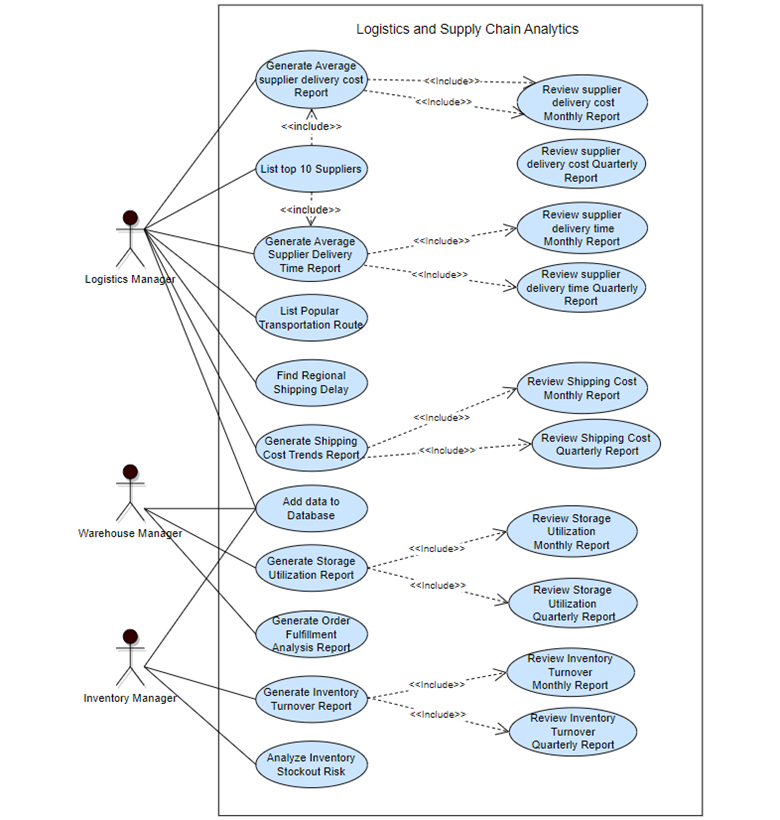
\includegraphics[width=1\textwidth]{UML.png} 
	\caption{Use Case Model}
	\label{fig:Use Case Model}
\end{figure}

\section{Use Cases}
\textbf{Actor Definitions:}
\begin{itemize}
	\item \textbf{Logistics Managers}: These users oversee transportation, shipping, and supplier operations and relation.
	\item \textbf{Warehouse Managers}: They manage warehouse operations, including storage space utilization and order fulfillment.
	\item \textbf{Inventory Managers}: These users are responsible for inventory management based on shipment and supplier information and turnover rate analysis.
\end{itemize}
\begin{center}
	\begin{tabularx}{\textwidth}{|l|X|}
		\hline
		System & METRICSTICS \\
		\hline
		Identifier & UC-1 \\
		\hline
		Author(s) & \begin{itemize}[left=0pt]
			\item Author Name: Sharanyu Pillai
			\item Author Email: sharanyu@hotmail.com
		\end{itemize} \\
		\hline
		Version & 1.0 \\
		\hline
		Priority & Medium \\
		\hline
		Name & Calculating Average supplier delivery cost for the stock procured \\
		\hline
		Pre-Condition(s) &  \begin{itemize}[left=0pt]
			\item User has a valid account on the system.
			\item Supply stock data is available in the system.
		\end{itemize} \\
		\hline
		Post-Condition(s) & \begin{itemize}[left=0pt]
			\item Average monthly and quarterly delivery cost report is generated.
		\end{itemize} \\
		\hline
		Trigger & Logistics Manager initiates the analysis. \\
		\hline
		Normal Flow & \begin{enumerate}[left=0pt]
			\item Logistics Manager logs into the system.
			\item Logistics Manager  selects the supply delivery cost analysis option.
			\item Logistics Manager  inputs new supply delivery cost data.
			\item System generates an analysis report.
		\end{enumerate} \\
		\hline
		Exceptional Flow & None \\
		\hline
		Related Actor(s) & Logistics Manager \\
		\hline
		Related Use Case(s) & None \\
		\hline
		Description & Logistics Manager averages shipping cost for the supply obtained monthly and quarterly to make improvements and reduce expenses in the future. \\
		\hline
	\end{tabularx}
\end{center}

\begin{center}
	\begin{tabularx}{\textwidth}{|l|X|}
		\hline
		System & METRICSTICS \\
		\hline
		Identifier & UC-2 \\
		\hline
		Author(s) & \begin{itemize}[left=0pt]
			\item Author Name: Sharanyu Pillai
			\item Author Email: sharanyu@hotmail.com
		\end{itemize} \\
		\hline
		Version & 1.0 \\
		\hline
		Priority & High \\
		\hline
		Name & Supplier Delivery Time Trends \\
		\hline
		Pre-Condition(s) &  \begin{itemize}[left=0pt]
			\item Valid user account in the system.
			\item Availability of supplier delivery time data.
		\end{itemize} \\
		\hline
		Post-Condition(s) & \begin{itemize}[left=0pt]
			\item Supplier delivery time trend report generated.
		\end{itemize} \\
		\hline
		Trigger & Logistics Manager initiates analysis. \\
		\hline
		Normal Flow & \begin{enumerate}[left=0pt]
			\item Logistics Manager logs in.
			\item Selects supplier delivery time trend analysis.
			\item Inputs delivery time data.
			\item System generates supplier delivery time trend.
		\end{enumerate} \\
		\hline
		Exceptional Flow & None \\
		\hline
		Related Actor(s) & Logistics Managers \\
		\hline
		Related Use Case(s) & None \\
		\hline
		Description & Logistics Managers analyze supplier delivery time trends to identify months and quarters with significant changes. \\
		\hline
	\end{tabularx}
\end{center}

\begin{center}
	\begin{tabularx}{\textwidth}{|l|X|}
		\hline
		System & METRICSTICS \\
		\hline
		Identifier & UC-3 \\
		\hline
		Author(s) & \begin{itemize}[left=0pt]
			\item Author Name: Wei Qi
			\item Author Email: qiwei12181@163.com
		\end{itemize} \\
		\hline
		Version & 1.0 \\
		\hline
		Priority & Moderate \\
		\hline
		Name & Shipping Cost Trend Analysis \\
		\hline
		Pre-Condition(s) &  \begin{itemize}[left=0pt]
			\item Valid user account in the system.
			\item Availability of shipping cost data.
		\end{itemize} \\
		\hline
		Post-Condition(s) & \begin{itemize}[left=0pt]
			\item Shipping cost trend report generated.
		\end{itemize} \\
		\hline
		Trigger & Logistics Manager initiates analysis. \\
		\hline
		Normal Flow & \begin{enumerate}[left=0pt]
			\item Logistics Manager logs in.
			\item Selects shipping cost trend analysis option.
			\item Inputs shipping cost data.
			\item System generates shipping cost trend report.
		\end{enumerate} \\
		\hline
		Exceptional Flow & None \\
		\hline
		Related Actor(s) & Logistics Managers \\
		\hline
		Related Use Case(s) & None \\
		\hline
		Description & Logistics Managers analyze shipping cost trends for each shipping method to optimize cost-effectiveness. \\
		\hline
	\end{tabularx}
\end{center}

\begin{center}
	\begin{tabularx}{\textwidth}{|l|X|}
		\hline
		System & METRICSTICS \\
		\hline
		Identifier & UC-4 \\
		\hline
		Author(s) & \begin{itemize}[left=0pt]
			\item Author Name: Wei Qi
			\item Author Email: qiwei12181@163.com
		\end{itemize} \\
		\hline
		Version & 1.0 \\
		\hline
		Priority & Moderate \\
		\hline
		Name & Storage Utilization Monitoring \\
		\hline
		Pre-Condition(s) &  \begin{itemize}[left=0pt]
			\item Valid user account in the system.
			\item Availability of warehouse storage data.
		\end{itemize} \\
		\hline
		Post-Condition(s) & \begin{itemize}[left=0pt]
			\item Storage utilization monitoring report generated.
		\end{itemize} \\
		\hline
		Trigger & Warehouse Manager initiates monitoring. \\
		\hline
		Normal Flow & \begin{enumerate}[left=0pt]
			\item Warehouse Manager logs in.
			\item Selects storage utilization monitoring option.
			\item Inputs storage utilization data.
			\item System generates storage utilization monitoring report.
		\end{enumerate} \\
		\hline
		Exceptional Flow & None \\
		\hline
		Related Actor(s) & Warehouse Managers \\
		\hline
		Related Use Case(s) & None \\
		\hline
		Description & Warehouse Managers monitor storage space utilization on a monthly and quarterly basis to identify fluctuations and optimize space allocation. \\
		\hline
	\end{tabularx}
\end{center}

\begin{center}
	\begin{tabularx}{\textwidth}{|l|X|}
		\hline
		System & METRICSTICS \\
		\hline
		Identifier & UC-5 \\
		\hline
		Author(s) & \begin{itemize}[left=0pt]
			\item Author Name: Anitha Ramakrishnan
			\item Author Email: anitha5685@gmail.com
		\end{itemize} \\
		\hline
		Version & 1.0 \\
		\hline
		Priority & Moderate \\
		\hline
		Name & Inventory Turnover Analysis \\
		\hline
		Pre-Condition(s) &  \begin{itemize}[left=0pt]
			\item Valid user account in the system.
			\item Availability of inventory turnover rate data.
		\end{itemize} \\
		\hline
		Post-Condition(s) & \begin{itemize}[left=0pt]
			\item Inventory turnover analysis report generated.
		\end{itemize} \\
		\hline
		Trigger & Inventory Manager initiates analysis. \\
		\hline
		Normal Flow & \begin{enumerate}[left=0pt]
			\item Inventory Manager logs in.
			\item Selects inventory turnover analysis option.
			\item Inputs turnover rate data.
			\item System generates inventory turnover analysis report.
		\end{enumerate} \\
		\hline
		Exceptional Flow & None \\
		\hline
		Related Actor(s) & Inventory Managers \\
		\hline
		Related Use Case(s) & None \\
		\hline
		Description & Inventory Managers analyze inventory turnover rates to identify months and quarters with significant changes. \\
		\hline
	\end{tabularx}
\end{center}

\begin{center}
	\begin{tabularx}{\textwidth}{|l|X|}
		\hline
		System & METRICSTICS \\
		\hline
		Identifier & UC-6 \\
		\hline
		Author(s) & \begin{itemize}[left=0pt]
			\item Author Name: Anitha Ramakrishnan
			\item Author Email: anitha5685@gmail.com
		\end{itemize} \\
		\hline
		Version & 1.0 \\
		\hline
		Priority & Moderate \\
		\hline
		Name & List top 10 Suppliers based on their Performance Ranking \\
		\hline
		Pre-Condition(s) &  \begin{itemize}[left=0pt]
			\item Valid user account in the system.
			\item Availability of supplier performance data.
		\end{itemize} \\
		\hline
		Post-Condition(s) & \begin{itemize}[left=0pt]
			\item Top 10 Supplier ranking list generated.
		\end{itemize} \\
		\hline
		Trigger & Logistics Manager initiates ranking. \\
		\hline
		Normal Flow & \begin{enumerate}[left=0pt]
			\item Logistics Manager logs in.
			\item Selects supplier performance ranking option.
			\item Utilizes inputs for supplier performance data.
			\item System generates supplier ranking report.
		\end{enumerate} \\
		\hline
		Exceptional Flow & None \\
		\hline
		Related Actor(s) & Logistics Managers \\
		\hline
		Related Use Case(s) & UC-1 and UC-2 \\
		\hline
		Description & Logistics Managers rank suppliers based on their on-time delivery performance and more affordable delivery cost on a monthly and quarterly basis. \\
		\hline
	\end{tabularx}
\end{center}

\begin{center}
	\begin{tabularx}{\textwidth}{|l|X|}
		\hline
		System & METRICSTICS \\
		\hline
		Identifier & UC-7 \\
		\hline
		Author(s) & \begin{itemize}[left=0pt]
			\item Author Name: Arshiya Sahni
			\item Author Email: arshiyasahni87@gmail.com
		\end{itemize} \\
		\hline
		Version & 1.0 \\
		\hline
		Priority & Moderate \\
		\hline
		Name & Analyzing Popular Transportation Routes \\
		\hline
		Pre-Condition(s) &  \begin{itemize}[left=0pt]
			\item Valid user account in the system.
			\item Availability of shipment route data.
		\end{itemize} \\
		\hline
		Post-Condition(s) & \begin{itemize}[left=0pt]
			\item Route analytics report generated.
		\end{itemize} \\
		\hline
		Trigger & Logistics Manager initiates analysis. \\
		\hline
		Normal Flow & \begin{enumerate}[left=0pt]
			\item Logistics Manager logs in.
			\item Selects route analytics option.
			\item Inputs shipment route data.
			\item System generates route analytics report.
		\end{enumerate} \\
		\hline
		Exceptional Flow & None \\
		\hline
		Related Actor(s) & Logistics Managers \\
		\hline
		Related Use Case(s) & None \\
		\hline
		Description & Logistics Managers analyze the popularity of transportation routes for shipments on a monthly basis. \\
		\hline
	\end{tabularx}
\end{center}

\begin{center}
	\begin{tabularx}{\textwidth}{|l|X|}
		\hline
		System & METRICSTICS \\
		\hline
		Identifier & UC-8 \\
		\hline
		Author(s) & \begin{itemize}[left=0pt]
			\item Author Name: Arshiya Sahni
			\item Author Email: arshiyasahni87@gmail.com
		\end{itemize} \\
		\hline
		Version & 1.0 \\
		\hline
		Priority & Low \\
		\hline
		Name & Calculating Regional Shipping Delay \\
		\hline
		Pre-Condition(s) &  \begin{itemize}[left=0pt]
			\item Valid user account in the system.
			\item Availability of shipping delay data.
		\end{itemize} \\
		\hline
		Post-Condition(s) & \begin{itemize}[left=0pt]
			\item Regional delay analysis report generated.
		\end{itemize} \\
		\hline
		Trigger & Logistics Manager initiates analysis. \\
		\hline
		Normal Flow & \begin{enumerate}[left=0pt]
			\item Logistics Manager logs in.
			\item Selects regional delay analysis option.
			\item Inputs shipping delay data.
			\item System generates regional delay analysis report.
		\end{enumerate} \\
		\hline
		Exceptional Flow & None \\
		\hline
		Related Actor(s) & Logistics Managers \\
		\hline
		Related Use Case(s) & None \\
		\hline
		Description & Logistics Managers analyze shipping delays by region on a yearly basis to identify regions with the highest delays. \\
		\hline
	\end{tabularx}
\end{center}

\begin{center}
	\begin{tabularx}{\textwidth}{|l|X|}
		\hline
		System & METRICSTICS \\
		\hline
		Identifier & UC-9 \\
		\hline
		Author(s) & \begin{itemize}[left=0pt]
			\item Author Name: Vinay Sahrawat
			\item Author Email: vinaysahrawat183a@gmail.com
		\end{itemize} \\
		\hline
		Version & 1.0 \\
		\hline
		Priority & High \\
		\hline
		Name & Assessing Inventory Stockout Risk \\
		\hline
		Pre-Condition(s) &  \begin{itemize}[left=0pt]
			\item Valid user account in the system.
			\item Availability of inventory data and demand forecasts.
		\end{itemize} \\
		\hline
		Post-Condition(s) & \begin{itemize}[left=0pt]
			\item Stockout risk assessment report generated.
		\end{itemize} \\
		\hline
		Trigger & Inventory Manager initiates assessment. \\
		\hline
		Normal Flow & \begin{enumerate}[left=0pt]
			\item Inventory Manager logs in.
			\item Selects stockout risk assessment option.
			\item Inputs inventory data and demand forecasts.
			\item System generates stockout risk assessment report.
		\end{enumerate} \\
		\hline
		Exceptional Flow & None \\
		\hline
		Related Actor(s) & Inventory Managers \\
		\hline
		Related Use Case(s) & None \\
		\hline
		Description & Inventory Managers assess the risk of stockouts by analyzing inventory levels and demand forecasts. \\
		\hline
	\end{tabularx}
\end{center}

\begin{center}
	\begin{tabularx}{\textwidth}{|l|X|}
		\hline
		System & METRICSTICS \\
		\hline
		Identifier & UC-10 \\
		\hline
		Author(s) & \begin{itemize}[left=0pt]
			\item Author Name: Vinay Sahrawat
			\item Author Email: vinaysahrawat183a@gmail.com
		\end{itemize} \\
		\hline
		Version & 1.0 \\
		\hline
		Priority & High \\
		\hline
		Name & Calculating number of orders fulfilled in a year \\
		\hline
		Pre-Condition(s) &  \begin{itemize}[left=0pt]
			\item Valid user account in the system.
			\item Availability of demand forecast and actual demand data.Availability of number of orders shipped from warehouse data.
		\end{itemize} \\
		\hline
		Post-Condition(s) & \begin{itemize}[left=0pt]
			\item Forecast accuracy analysis report generated.
		\end{itemize} \\
		\hline
		Trigger & Warehouse Manager initiates analysis. \\
		\hline
		Normal Flow & \begin{enumerate}[left=0pt]
			\item Warehouse Manager logs in.
			\item Selects numbers of order shipped option.
			\item Inputs format of viewing report data.
			\item System generates analysis report for order fulfillment.
		\end{enumerate} \\
		\hline
		Exceptional Flow & None \\
		\hline
		Related Actor(s) & Warehouse Managers \\
		\hline
		Related Use Case(s) & None \\
		\hline
		Description & Warehouse Managers analyze the shipped order number from the warehouse and generate a report. \\
		\hline
	\end{tabularx}
\end{center}





	
	\chapter{Team Contribution}
	\section{Team Members and Roles}
	\begin{center}
		\begin{tabular}{|l|p{0.4\linewidth}|l|}
			\hline
			\textbf{Team Member} & \textbf{Roles}\\
			\hline
			Sharanyu Pillai (40227794) & 2 Metric Questions, Actor Definitions and Use Case Descriptions, Introduction\\
			\hline
			Arshiya Sahni (40202614) & 2 Metric Questions, Actor Definitions and Use Case Descriptions, Use Case Diagram\\
			\hline
			Anitha Ramakrishnan (40231724) & 2 Metric Questions, Actor Definitions and Use Case Descriptions\\
			\hline
			Vinay Sahrawat (40220936) & 2 Metric Questions, Actor Definitions and Use Case Descriptions\\
			\hline
			Wei Qi (40198872) & 2 Metric Questions, Actor Definitions and Use Case Descriptions, Latex Compilation \\
			\hline
		\end{tabular}
	\end{center}

	\chapter{Reference}
	\begin{enumerate}
	\item https://www.leadingagile.com/2017/05/agile-metrics-gqm-approach
	\item https://www.geeksforgeeks.org/software-measurement-and-metrics
	\item https://www.wrike.com/project-management-guide/faq/what-is-smart-in-project-management/ 
	
	\end{enumerate}
	
	

\end{document}
